\NeedsTeXFormat{LaTeX2e}
\documentclass[a4paper,11pt]{article}
\usepackage[utf8]{inputenc}

\usepackage[affil-it]{authblk}

%\usepackage{layouts}
\usepackage{setspace}

\usepackage{booktabs}
\usepackage{amsmath}
\usepackage{amssymb}
\usepackage{epsfig}

\usepackage{marvosym}

\usepackage{graphicx}
\usepackage{caption}
\usepackage{subcaption}
\usepackage{multicol}
\usepackage{etoolbox}

\usepackage{todonotes}

\usepackage{tikz}

\setlength{\textheight}{9in}
\setlength{\textwidth}{6in}
\setlength{\oddsidemargin}{.25in}
\setlength{\topmargin}{-.5in} 

\patchcmd{\thebibliography}{\section*{\refname}}
    {\begin{multicols}{2}[\section*{\refname}\singlespace\footnotesize]}{}{}
\patchcmd{\endthebibliography}{\endlist}{\endlist\end{multicols}}{}{}

\hyphenation{itself}

\title{{\small 02935 Introduction to applied statistics and R for PhD students: }\\[1em]Project report: Weather and travel demand}

\author{Niklas Christoffer Petersen}
\affil{Transport Modelling, Department of Management Engineering \\ Technical University of Denmark, 2800 Kongens Lyngby, Denmark}

%\affil{Trafikselskabet Movia \\ Technical University of Denmark, 2800 Kongens Lyngby, Denmark}

\begin{document}
\singlespace
\maketitle
\thispagestyle{empty}
\clearpage

\onehalfspacing
\pagenumbering{arabic}
\tableofcontents
\clearpage

\section{Background}\label{ch:background}

Observing and predicting the demand for bus travel is of major impact for designing and operating an efficient public transport system in any urban area. It is a common understanding, that there are several external factors that impact the travel demand. Examples include weather, events, etc. It is however uncertain how much each factor really contributes to fluctuation in travel demand. 

\subsection{Related work}\label{ch:relatedWork}
The impact of weather conditions on transport is a well-studied area within the scientific field of transport modeling.
TODO
\clearpage

\section{Data acquisition and preparation}\label{ch:data}
As established earlier, the goal of this project is to shed light upon the impact of specifically weather as an external factor for bus travel demand. For this, both historical weather data, and measures of historical travel demand should be obtained and prepared.

\subsection{Historical weather data}\label{ch:data_weather}
Historical weather data are unfortunately often still considered an asset, and therefore rarely public accessible in detailed granularity. Even though the Danish government has opened a lot of public data, and made them accessible for free use, data from the Danish Meteorological Institute (DMI) is still not freely available.

\emph{Weather Underground}\footnote{https://www.wunderground.com/} provides world covering weather forecasts and therefore has huge amount of historical weather data. They have an API, which also includes a free student/research plan, which gives (limited) access to historical weather data. Because the API only allows querying for on day at a time, a small \emph{Python} script was written to scrap the API for 6 months of historical weather data between October 2017 and March 2017.

\subsection{Travel demand data}\label{ch:data_traveldemand}
Getting a appropriate measures of travel demand is a non-trivial task in itself\todo{cite?}. For this project two data sources was considered:
\begin{itemize}
	\item The Danish national smart-card ticketing system, \emph{Rejsekort}, which is installed in every vehicle. Boardings are recorded as passengers \emph{check in} using their smart-card.
	\item The camera-based \emph{automatic people counting} (APC) systems that are installed in a subset of vehicles. Boardings are recorded using image analysis of cameras mounted over the doors.
\end{itemize}

Both systems has limitations though. Obviously the APC system suffers from only measuring a small sample ($<8\%$ of departures), and thus the the chance of having measurements for extreme weather conditions is reduced.

On the other hand, boarding data from the Danish national smart-card ticketing system, \emph{Rejsekort}, is installed in every vehicle. But as several other ticket types are also available (Cash-tickets, Season Passes, Mobile Apps, etc.), it does not give a complete boarding measure. Compared to the sample from the APC system, the smart-card ticketing system only accounts for~$\approx 24\%$ of passenger boardings.

\todo{Connect}

Data from the smart-card ticketing system for the period between October 2017 and March 2017 was selected.

\section{Data description}\label{ch:desc}

\subsection{Travel demand data}\label{ch:desc_traveldemand}

Obviously travel demand varies throughout the day, with p
\begin{figure}[!ht]
	\center
	%\includegraphics{../plots/travelcard_hist.pdf}
	% !TEX encoding = UTF-8 Unicode
\begin{tikzpicture}[x=1pt,y=1pt]
\definecolor{fillColor}{RGB}{255,255,255}
\path[use as bounding box,fill=fillColor,fill opacity=0.00] (0,0) rectangle (433.62,216.81);
\begin{scope}
\path[clip] (  0.00,  0.00) rectangle (433.62,216.81);
\definecolor{drawColor}{RGB}{255,255,255}
\definecolor{fillColor}{RGB}{255,255,255}

\path[draw=drawColor,line width= 0.6pt,line join=round,line cap=round,fill=fillColor] (  0.00,  0.00) rectangle (433.62,216.81);
\end{scope}
\begin{scope}
\path[clip] ( 47.21, 34.62) rectangle (427.62,210.81);
\definecolor{fillColor}{RGB}{255,255,255}

\path[fill=fillColor] ( 47.21, 34.62) rectangle (427.62,210.81);
\definecolor{drawColor}{gray}{0.98}

\path[draw=drawColor,line width= 0.6pt,line join=round] ( 47.21, 66.84) --
	(427.62, 66.84);

\path[draw=drawColor,line width= 0.6pt,line join=round] ( 47.21,116.24) --
	(427.62,116.24);

\path[draw=drawColor,line width= 0.6pt,line join=round] ( 47.21,165.65) --
	(427.62,165.65);
\definecolor{drawColor}{gray}{0.90}

\path[draw=drawColor,line width= 0.2pt,line join=round] ( 47.21, 42.14) --
	(427.62, 42.14);

\path[draw=drawColor,line width= 0.2pt,line join=round] ( 47.21, 91.54) --
	(427.62, 91.54);

\path[draw=drawColor,line width= 0.2pt,line join=round] ( 47.21,140.95) --
	(427.62,140.95);

\path[draw=drawColor,line width= 0.2pt,line join=round] ( 47.21,190.35) --
	(427.62,190.35);

\path[draw=drawColor,line width= 0.2pt,line join=round] ( 78.91, 34.62) --
	( 78.91,210.81);

\path[draw=drawColor,line width= 0.2pt,line join=round] (131.74, 34.62) --
	(131.74,210.81);

\path[draw=drawColor,line width= 0.2pt,line join=round] (184.58, 34.62) --
	(184.58,210.81);

\path[draw=drawColor,line width= 0.2pt,line join=round] (237.41, 34.62) --
	(237.41,210.81);

\path[draw=drawColor,line width= 0.2pt,line join=round] (290.25, 34.62) --
	(290.25,210.81);

\path[draw=drawColor,line width= 0.2pt,line join=round] (343.08, 34.62) --
	(343.08,210.81);

\path[draw=drawColor,line width= 0.2pt,line join=round] (395.92, 34.62) --
	(395.92,210.81);
\definecolor{drawColor}{RGB}{248,118,109}

\path[draw=drawColor,line width= 0.6pt,line join=round] ( 78.91,125.24) -- ( 78.91,190.85);

\path[draw=drawColor,line width= 0.6pt,line join=round] ( 78.91, 55.72) -- ( 78.91, 42.93);

\path[draw=drawColor,line width= 0.6pt,line join=round,line cap=round,fill=fillColor] ( 59.10,125.24) --
	( 59.10,100.72) --
	( 69.00, 96.24) --
	( 59.10, 91.75) --
	( 59.10, 55.72) --
	( 98.72, 55.72) --
	( 98.72, 91.75) --
	( 88.81, 96.24) --
	( 98.72,100.72) --
	( 98.72,125.24) --
	( 59.10,125.24) --
	cycle;

\path[draw=drawColor,line width= 1.1pt,line join=round] ( 69.00, 96.24) -- ( 88.81, 96.24);
\definecolor{drawColor}{RGB}{196,154,0}

\path[draw=drawColor,line width= 0.6pt,line join=round] (131.74,125.83) -- (131.74,181.76);

\path[draw=drawColor,line width= 0.6pt,line join=round] (131.74, 56.64) -- (131.74, 42.63);

\path[draw=drawColor,line width= 0.6pt,line join=round,line cap=round,fill=fillColor] (111.93,125.83) --
	(111.93,103.71) --
	(121.84, 99.25) --
	(111.93, 94.79) --
	(111.93, 56.64) --
	(151.56, 56.64) --
	(151.56, 94.79) --
	(141.65, 99.25) --
	(151.56,103.71) --
	(151.56,125.83) --
	(111.93,125.83) --
	cycle;

\path[draw=drawColor,line width= 1.1pt,line join=round] (121.84, 99.25) -- (141.65, 99.25);
\definecolor{drawColor}{RGB}{83,180,0}

\path[draw=drawColor,line width= 0.6pt,line join=round] (184.58,128.10) -- (184.58,193.51);

\path[draw=drawColor,line width= 0.6pt,line join=round] (184.58, 58.24) -- (184.58, 42.93);

\path[draw=drawColor,line width= 0.6pt,line join=round,line cap=round,fill=fillColor] (164.77,128.10) --
	(164.77,104.94) --
	(174.67,100.44) --
	(164.77, 95.93) --
	(164.77, 58.24) --
	(204.39, 58.24) --
	(204.39, 95.93) --
	(194.49,100.44) --
	(204.39,104.94) --
	(204.39,128.10) --
	(164.77,128.10) --
	cycle;

\path[draw=drawColor,line width= 1.1pt,line join=round] (174.67,100.44) -- (194.49,100.44);
\definecolor{drawColor}{RGB}{0,192,148}

\path[draw=drawColor,line width= 0.6pt,line join=round] (237.41,129.88) -- (237.41,202.80);

\path[draw=drawColor,line width= 0.6pt,line join=round] (237.41, 59.55) -- (237.41, 43.03);

\path[draw=drawColor,line width= 0.6pt,line join=round,line cap=round,fill=fillColor] (217.60,129.88) --
	(217.60,107.34) --
	(227.51,102.81) --
	(217.60, 98.27) --
	(217.60, 59.55) --
	(257.23, 59.55) --
	(257.23, 98.27) --
	(247.32,102.81) --
	(257.23,107.34) --
	(257.23,129.88) --
	(217.60,129.88) --
	cycle;

\path[draw=drawColor,line width= 1.1pt,line join=round] (227.51,102.81) -- (247.32,102.81);
\definecolor{drawColor}{RGB}{0,182,235}

\path[draw=drawColor,line width= 0.6pt,line join=round] (290.25,139.96) -- (290.25,199.94);

\path[draw=drawColor,line width= 0.6pt,line join=round] (290.25, 69.85) -- (290.25, 44.02);

\path[draw=drawColor,line width= 0.6pt,line join=round,line cap=round,fill=fillColor] (270.44,139.96) --
	(270.44,115.67) --
	(280.34,111.06) --
	(270.44,106.44) --
	(270.44, 69.85) --
	(310.06, 69.85) --
	(310.06,106.44) --
	(300.16,111.06) --
	(310.06,115.67) --
	(310.06,139.96) --
	(270.44,139.96) --
	cycle;

\path[draw=drawColor,line width= 1.1pt,line join=round] (280.34,111.06) -- (300.16,111.06);
\definecolor{drawColor}{RGB}{165,138,255}

\path[draw=drawColor,line width= 0.6pt,line join=round] (343.08,132.99) -- (343.08,175.83);

\path[draw=drawColor,line width= 0.6pt,line join=round] (343.08, 64.67) -- (343.08, 47.87);

\path[draw=drawColor,line width= 0.6pt,line join=round,line cap=round,fill=fillColor] (323.27,132.99) --
	(323.27, 97.47) --
	(333.18, 92.98) --
	(323.27, 88.48) --
	(323.27, 64.67) --
	(362.90, 64.67) --
	(362.90, 88.48) --
	(352.99, 92.98) --
	(362.90, 97.47) --
	(362.90,132.99) --
	(323.27,132.99) --
	cycle;

\path[draw=drawColor,line width= 1.1pt,line join=round] (333.18, 92.98) -- (352.99, 92.98);
\definecolor{drawColor}{RGB}{251,97,215}

\path[draw=drawColor,line width= 0.6pt,line join=round] (395.92,108.98) -- (395.92,143.81);

\path[draw=drawColor,line width= 0.6pt,line join=round] (395.92, 59.31) -- (395.92, 47.18);

\path[draw=drawColor,line width= 0.6pt,line join=round,line cap=round,fill=fillColor] (376.11,108.98) --
	(376.11, 80.34) --
	(386.01, 77.07) --
	(376.11, 73.80) --
	(376.11, 59.31) --
	(415.73, 59.31) --
	(415.73, 73.80) --
	(405.83, 77.07) --
	(415.73, 80.34) --
	(415.73,108.98) --
	(376.11,108.98) --
	cycle;

\path[draw=drawColor,line width= 1.1pt,line join=round] (386.01, 77.07) -- (405.83, 77.07);
\definecolor{drawColor}{gray}{0.50}

\path[draw=drawColor,line width= 0.6pt,line join=round,line cap=round] ( 47.21, 34.62) rectangle (427.62,210.81);
\end{scope}
\begin{scope}
\path[clip] (  0.00,  0.00) rectangle (433.62,216.81);
\definecolor{drawColor}{RGB}{0,0,0}

\node[text=drawColor,anchor=base east,inner sep=0pt, outer sep=0pt, scale=  0.96] at ( 41.81, 38.83) {0};

\node[text=drawColor,anchor=base east,inner sep=0pt, outer sep=0pt, scale=  0.96] at ( 41.81, 88.24) {500};

\node[text=drawColor,anchor=base east,inner sep=0pt, outer sep=0pt, scale=  0.96] at ( 41.81,137.64) {1000};

\node[text=drawColor,anchor=base east,inner sep=0pt, outer sep=0pt, scale=  0.96] at ( 41.81,187.05) {1500};
\end{scope}
\begin{scope}
\path[clip] (  0.00,  0.00) rectangle (433.62,216.81);
\definecolor{drawColor}{RGB}{0,0,0}

\path[draw=drawColor,line width= 0.6pt,line join=round] ( 44.21, 42.14) --
	( 47.21, 42.14);

\path[draw=drawColor,line width= 0.6pt,line join=round] ( 44.21, 91.54) --
	( 47.21, 91.54);

\path[draw=drawColor,line width= 0.6pt,line join=round] ( 44.21,140.95) --
	( 47.21,140.95);

\path[draw=drawColor,line width= 0.6pt,line join=round] ( 44.21,190.35) --
	( 47.21,190.35);
\end{scope}
\begin{scope}
\path[clip] (  0.00,  0.00) rectangle (433.62,216.81);
\definecolor{drawColor}{RGB}{0,0,0}

\path[draw=drawColor,line width= 0.6pt,line join=round] ( 78.91, 31.62) --
	( 78.91, 34.62);

\path[draw=drawColor,line width= 0.6pt,line join=round] (131.74, 31.62) --
	(131.74, 34.62);

\path[draw=drawColor,line width= 0.6pt,line join=round] (184.58, 31.62) --
	(184.58, 34.62);

\path[draw=drawColor,line width= 0.6pt,line join=round] (237.41, 31.62) --
	(237.41, 34.62);

\path[draw=drawColor,line width= 0.6pt,line join=round] (290.25, 31.62) --
	(290.25, 34.62);

\path[draw=drawColor,line width= 0.6pt,line join=round] (343.08, 31.62) --
	(343.08, 34.62);

\path[draw=drawColor,line width= 0.6pt,line join=round] (395.92, 31.62) --
	(395.92, 34.62);
\end{scope}
\begin{scope}
\path[clip] (  0.00,  0.00) rectangle (433.62,216.81);
\definecolor{drawColor}{RGB}{0,0,0}

\node[text=drawColor,anchor=base,inner sep=0pt, outer sep=0pt, scale=  0.96] at ( 78.91, 22.61) {Mon};

\node[text=drawColor,anchor=base,inner sep=0pt, outer sep=0pt, scale=  0.96] at (131.74, 22.61) {Tue};

\node[text=drawColor,anchor=base,inner sep=0pt, outer sep=0pt, scale=  0.96] at (184.58, 22.61) {Wed};

\node[text=drawColor,anchor=base,inner sep=0pt, outer sep=0pt, scale=  0.96] at (237.41, 22.61) {Thu};

\node[text=drawColor,anchor=base,inner sep=0pt, outer sep=0pt, scale=  0.96] at (290.25, 22.61) {Fri};

\node[text=drawColor,anchor=base,inner sep=0pt, outer sep=0pt, scale=  0.96] at (343.08, 22.61) {Sat};

\node[text=drawColor,anchor=base,inner sep=0pt, outer sep=0pt, scale=  0.96] at (395.92, 22.61) {Sun};
\end{scope}
\begin{scope}
\path[clip] (  0.00,  0.00) rectangle (433.62,216.81);
\definecolor{drawColor}{RGB}{0,0,0}

\node[text=drawColor,anchor=base,inner sep=0pt, outer sep=0pt, scale=  0.96] at (237.41,  6.00) {Day of week, $\mathit{dow}$};
\end{scope}
\begin{scope}
\path[clip] (  0.00,  0.00) rectangle (433.62,216.81);
\definecolor{drawColor}{RGB}{0,0,0}

\node[text=drawColor,rotate= 90.00,anchor=base,inner sep=0pt, outer sep=0pt, scale=  0.96] at ( 12.61,122.72) {Travel demand, $D$};
\end{scope}
\end{tikzpicture}

	\caption{Passenger boardings by day of week.}
\end{figure}

more

\begin{figure}[!ht]
	\center
	%\includegraphics{../plots/travelcard_hist.pdf}
	% !TEX encoding = UTF-8 Unicode
\begin{tikzpicture}[x=1pt,y=1pt]
\definecolor{fillColor}{RGB}{255,255,255}
\path[use as bounding box,fill=fillColor,fill opacity=0.00] (0,0) rectangle (433.62,216.81);
\begin{scope}
\path[clip] (  0.00,  0.00) rectangle (433.62,216.81);
\definecolor{drawColor}{RGB}{255,255,255}
\definecolor{fillColor}{RGB}{255,255,255}

\path[draw=drawColor,line width= 0.6pt,line join=round,line cap=round,fill=fillColor] (  0.00,  0.00) rectangle (433.62,216.81);
\end{scope}
\begin{scope}
\path[clip] ( 47.21, 74.69) rectangle (427.62,210.81);
\definecolor{fillColor}{RGB}{255,255,255}

\path[fill=fillColor] ( 47.21, 74.69) rectangle (427.62,210.81);
\definecolor{drawColor}{gray}{0.98}

\path[draw=drawColor,line width= 0.6pt,line join=round] ( 47.21,103.64) --
	(427.62,103.64);

\path[draw=drawColor,line width= 0.6pt,line join=round] ( 47.21,152.33) --
	(427.62,152.33);

\path[draw=drawColor,line width= 0.6pt,line join=round] ( 47.21,201.01) --
	(427.62,201.01);

\path[draw=drawColor,line width= 0.6pt,line join=round] ( 49.46, 74.69) --
	( 49.46,210.81);

\path[draw=drawColor,line width= 0.6pt,line join=round] ( 64.50, 74.69) --
	( 64.50,210.81);

\path[draw=drawColor,line width= 0.6pt,line join=round] ( 79.53, 74.69) --
	( 79.53,210.81);

\path[draw=drawColor,line width= 0.6pt,line join=round] ( 94.57, 74.69) --
	( 94.57,210.81);

\path[draw=drawColor,line width= 0.6pt,line join=round] (109.61, 74.69) --
	(109.61,210.81);

\path[draw=drawColor,line width= 0.6pt,line join=round] (124.64, 74.69) --
	(124.64,210.81);

\path[draw=drawColor,line width= 0.6pt,line join=round] (139.68, 74.69) --
	(139.68,210.81);

\path[draw=drawColor,line width= 0.6pt,line join=round] (154.72, 74.69) --
	(154.72,210.81);

\path[draw=drawColor,line width= 0.6pt,line join=round] (169.75, 74.69) --
	(169.75,210.81);

\path[draw=drawColor,line width= 0.6pt,line join=round] (184.79, 74.69) --
	(184.79,210.81);

\path[draw=drawColor,line width= 0.6pt,line join=round] (199.82, 74.69) --
	(199.82,210.81);

\path[draw=drawColor,line width= 0.6pt,line join=round] (214.86, 74.69) --
	(214.86,210.81);

\path[draw=drawColor,line width= 0.6pt,line join=round] (229.90, 74.69) --
	(229.90,210.81);

\path[draw=drawColor,line width= 0.6pt,line join=round] (244.93, 74.69) --
	(244.93,210.81);

\path[draw=drawColor,line width= 0.6pt,line join=round] (259.97, 74.69) --
	(259.97,210.81);

\path[draw=drawColor,line width= 0.6pt,line join=round] (275.00, 74.69) --
	(275.00,210.81);

\path[draw=drawColor,line width= 0.6pt,line join=round] (290.04, 74.69) --
	(290.04,210.81);

\path[draw=drawColor,line width= 0.6pt,line join=round] (305.08, 74.69) --
	(305.08,210.81);

\path[draw=drawColor,line width= 0.6pt,line join=round] (320.11, 74.69) --
	(320.11,210.81);

\path[draw=drawColor,line width= 0.6pt,line join=round] (335.15, 74.69) --
	(335.15,210.81);

\path[draw=drawColor,line width= 0.6pt,line join=round] (350.18, 74.69) --
	(350.18,210.81);

\path[draw=drawColor,line width= 0.6pt,line join=round] (365.22, 74.69) --
	(365.22,210.81);

\path[draw=drawColor,line width= 0.6pt,line join=round] (380.26, 74.69) --
	(380.26,210.81);

\path[draw=drawColor,line width= 0.6pt,line join=round] (395.29, 74.69) --
	(395.29,210.81);

\path[draw=drawColor,line width= 0.6pt,line join=round] (410.33, 74.69) --
	(410.33,210.81);

\path[draw=drawColor,line width= 0.6pt,line join=round] (425.36, 74.69) --
	(425.36,210.81);
\definecolor{drawColor}{gray}{0.90}

\path[draw=drawColor,line width= 0.2pt,line join=round] ( 47.21, 79.30) --
	(427.62, 79.30);

\path[draw=drawColor,line width= 0.2pt,line join=round] ( 47.21,127.98) --
	(427.62,127.98);

\path[draw=drawColor,line width= 0.2pt,line join=round] ( 47.21,176.67) --
	(427.62,176.67);

\path[draw=drawColor,line width= 0.2pt,line join=round] ( 56.98, 74.69) --
	( 56.98,210.81);

\path[draw=drawColor,line width= 0.2pt,line join=round] ( 72.02, 74.69) --
	( 72.02,210.81);

\path[draw=drawColor,line width= 0.2pt,line join=round] ( 87.05, 74.69) --
	( 87.05,210.81);

\path[draw=drawColor,line width= 0.2pt,line join=round] (102.09, 74.69) --
	(102.09,210.81);

\path[draw=drawColor,line width= 0.2pt,line join=round] (117.12, 74.69) --
	(117.12,210.81);

\path[draw=drawColor,line width= 0.2pt,line join=round] (132.16, 74.69) --
	(132.16,210.81);

\path[draw=drawColor,line width= 0.2pt,line join=round] (147.20, 74.69) --
	(147.20,210.81);

\path[draw=drawColor,line width= 0.2pt,line join=round] (162.23, 74.69) --
	(162.23,210.81);

\path[draw=drawColor,line width= 0.2pt,line join=round] (177.27, 74.69) --
	(177.27,210.81);

\path[draw=drawColor,line width= 0.2pt,line join=round] (192.31, 74.69) --
	(192.31,210.81);

\path[draw=drawColor,line width= 0.2pt,line join=round] (207.34, 74.69) --
	(207.34,210.81);

\path[draw=drawColor,line width= 0.2pt,line join=round] (222.38, 74.69) --
	(222.38,210.81);

\path[draw=drawColor,line width= 0.2pt,line join=round] (237.41, 74.69) --
	(237.41,210.81);

\path[draw=drawColor,line width= 0.2pt,line join=round] (252.45, 74.69) --
	(252.45,210.81);

\path[draw=drawColor,line width= 0.2pt,line join=round] (267.49, 74.69) --
	(267.49,210.81);

\path[draw=drawColor,line width= 0.2pt,line join=round] (282.52, 74.69) --
	(282.52,210.81);

\path[draw=drawColor,line width= 0.2pt,line join=round] (297.56, 74.69) --
	(297.56,210.81);

\path[draw=drawColor,line width= 0.2pt,line join=round] (312.59, 74.69) --
	(312.59,210.81);

\path[draw=drawColor,line width= 0.2pt,line join=round] (327.63, 74.69) --
	(327.63,210.81);

\path[draw=drawColor,line width= 0.2pt,line join=round] (342.67, 74.69) --
	(342.67,210.81);

\path[draw=drawColor,line width= 0.2pt,line join=round] (357.70, 74.69) --
	(357.70,210.81);

\path[draw=drawColor,line width= 0.2pt,line join=round] (372.74, 74.69) --
	(372.74,210.81);

\path[draw=drawColor,line width= 0.2pt,line join=round] (387.77, 74.69) --
	(387.77,210.81);

\path[draw=drawColor,line width= 0.2pt,line join=round] (402.81, 74.69) --
	(402.81,210.81);

\path[draw=drawColor,line width= 0.2pt,line join=round] (417.85, 74.69) --
	(417.85,210.81);
\definecolor{drawColor}{RGB}{248,118,109}

\path[draw=drawColor,line width= 0.6pt,line join=round] ( 64.50, 84.64) --
	( 79.53, 82.05) --
	( 94.57, 81.07) --
	(109.61, 80.89) --
	(124.64, 83.78) --
	(139.68, 90.86) --
	(154.72,113.43) --
	(169.75,161.03) --
	(184.79,176.70) --
	(199.82,146.43) --
	(214.86,144.67) --
	(229.90,154.30) --
	(244.93,159.82) --
	(259.97,158.93) --
	(275.00,171.29) --
	(290.04,187.31) --
	(305.08,186.71) --
	(320.11,166.88) --
	(335.15,146.23) --
	(350.18,127.59) --
	(365.22,116.98) --
	(380.26,114.86) --
	(395.29,106.26) --
	(410.33, 95.58);
\definecolor{drawColor}{RGB}{196,154,0}

\path[draw=drawColor,line width= 0.6pt,line join=round] ( 64.50, 87.70) --
	( 79.53, 81.97) --
	( 94.57, 80.87) --
	(109.61, 80.93) --
	(124.64, 83.10) --
	(139.68, 89.22) --
	(154.72,110.32) --
	(169.75,162.55) --
	(184.79,174.61) --
	(199.82,151.71) --
	(214.86,144.18) --
	(229.90,153.97) --
	(244.93,158.56) --
	(259.97,161.23) --
	(275.00,172.06) --
	(290.04,189.62) --
	(305.08,187.24) --
	(320.11,170.19) --
	(335.15,149.71) --
	(350.18,130.67) --
	(365.22,120.90) --
	(380.26,118.00) --
	(395.29,110.59) --
	(410.33, 98.07);
\definecolor{drawColor}{RGB}{83,180,0}

\path[draw=drawColor,line width= 0.6pt,line join=round] ( 64.50, 89.20) --
	( 79.53, 82.91) --
	( 94.57, 81.12) --
	(109.61, 81.29) --
	(124.64, 83.29) --
	(139.68, 90.37) --
	(154.72,112.04) --
	(169.75,164.04) --
	(184.79,177.70) --
	(199.82,150.74) --
	(214.86,144.16) --
	(229.90,153.40) --
	(244.93,161.15) --
	(259.97,163.00) --
	(275.00,173.59) --
	(290.04,190.76) --
	(305.08,194.00) --
	(320.11,175.71) --
	(335.15,150.60) --
	(350.18,132.46) --
	(365.22,122.86) --
	(380.26,120.29) --
	(395.29,114.71) --
	(410.33, 99.06);
\definecolor{drawColor}{RGB}{0,192,148}

\path[draw=drawColor,line width= 0.6pt,line join=round] ( 64.50, 89.72) --
	( 79.53, 83.35) --
	( 94.57, 81.36) --
	(109.61, 81.42) --
	(124.64, 83.81) --
	(139.68, 90.49) --
	(154.72,113.10) --
	(169.75,164.04) --
	(184.79,178.42) --
	(199.82,150.97) --
	(214.86,145.02) --
	(229.90,155.43) --
	(244.93,161.27) --
	(259.97,164.71) --
	(275.00,176.91) --
	(290.04,191.63) --
	(305.08,193.54) --
	(320.11,177.78) --
	(335.15,157.14) --
	(350.18,135.01) --
	(365.22,124.79) --
	(380.26,122.54) --
	(395.29,118.23) --
	(410.33,102.94);
\definecolor{drawColor}{RGB}{0,182,235}

\path[draw=drawColor,line width= 0.6pt,line join=round] ( 64.50, 92.92) --
	( 79.53, 85.16) --
	( 94.57, 83.17) --
	(109.61, 82.37) --
	(124.64, 84.93) --
	(139.68, 91.59) --
	(154.72,115.40) --
	(169.75,170.42) --
	(184.79,184.55) --
	(199.82,150.76) --
	(214.86,149.56) --
	(229.90,160.50) --
	(244.93,169.94) --
	(259.97,175.29) --
	(275.00,189.44) --
	(290.04,200.49) --
	(305.08,204.62) --
	(320.11,195.54) --
	(335.15,168.75) --
	(350.18,152.69) --
	(365.22,137.98) --
	(380.26,125.99) --
	(395.29,130.57) --
	(410.33,125.25);
\definecolor{drawColor}{RGB}{165,138,255}

\path[draw=drawColor,line width= 0.6pt,line join=round] ( 64.50,116.59) --
	( 79.53,101.92) --
	( 94.57, 99.92) --
	(109.61, 99.30) --
	(124.64, 94.18) --
	(139.68, 91.55) --
	(154.72, 87.68) --
	(169.75, 92.46) --
	(184.79,106.59) --
	(199.82,128.37) --
	(214.86,147.19) --
	(229.90,162.79) --
	(244.93,175.66) --
	(259.97,183.05) --
	(275.00,179.64) --
	(290.04,184.44) --
	(305.08,183.80) --
	(320.11,188.12) --
	(335.15,165.75) --
	(350.18,143.61) --
	(365.22,136.43) --
	(380.26,126.33) --
	(395.29,126.07) --
	(410.33,124.13);
\definecolor{drawColor}{RGB}{251,97,215}

\path[draw=drawColor,line width= 0.6pt,line join=round] ( 64.50,114.63) --
	( 79.53,101.59) --
	( 94.57,101.74) --
	(109.61, 96.37) --
	(124.64, 95.15) --
	(139.68, 90.81) --
	(154.72, 86.33) --
	(169.75, 86.99) --
	(184.79, 93.76) --
	(199.82,111.85) --
	(214.86,125.75) --
	(229.90,136.90) --
	(244.93,150.29) --
	(259.97,157.12) --
	(275.00,155.42) --
	(290.04,157.55) --
	(305.08,161.01) --
	(320.11,154.47) --
	(335.15,144.36) --
	(350.18,124.51) --
	(365.22,116.52) --
	(380.26,111.03) --
	(395.29,104.88) --
	(410.33, 94.65);
\definecolor{drawColor}{gray}{0.50}

\path[draw=drawColor,line width= 0.6pt,line join=round,line cap=round] ( 47.21, 74.69) rectangle (427.62,210.81);
\end{scope}
\begin{scope}
\path[clip] (  0.00,  0.00) rectangle (433.62,216.81);
\definecolor{drawColor}{RGB}{0,0,0}

\node[text=drawColor,anchor=base east,inner sep=0pt, outer sep=0pt, scale=  0.96] at ( 41.81, 76.00) {0};

\node[text=drawColor,anchor=base east,inner sep=0pt, outer sep=0pt, scale=  0.96] at ( 41.81,124.68) {500};

\node[text=drawColor,anchor=base east,inner sep=0pt, outer sep=0pt, scale=  0.96] at ( 41.81,173.36) {1000};
\end{scope}
\begin{scope}
\path[clip] (  0.00,  0.00) rectangle (433.62,216.81);
\definecolor{drawColor}{RGB}{0,0,0}

\path[draw=drawColor,line width= 0.6pt,line join=round] ( 44.21, 79.30) --
	( 47.21, 79.30);

\path[draw=drawColor,line width= 0.6pt,line join=round] ( 44.21,127.98) --
	( 47.21,127.98);

\path[draw=drawColor,line width= 0.6pt,line join=round] ( 44.21,176.67) --
	( 47.21,176.67);
\end{scope}
\begin{scope}
\path[clip] (  0.00,  0.00) rectangle (433.62,216.81);
\definecolor{drawColor}{RGB}{0,0,0}

\path[draw=drawColor,line width= 0.6pt,line join=round] ( 56.98, 71.69) --
	( 56.98, 74.69);

\path[draw=drawColor,line width= 0.6pt,line join=round] ( 72.02, 71.69) --
	( 72.02, 74.69);

\path[draw=drawColor,line width= 0.6pt,line join=round] ( 87.05, 71.69) --
	( 87.05, 74.69);

\path[draw=drawColor,line width= 0.6pt,line join=round] (102.09, 71.69) --
	(102.09, 74.69);

\path[draw=drawColor,line width= 0.6pt,line join=round] (117.12, 71.69) --
	(117.12, 74.69);

\path[draw=drawColor,line width= 0.6pt,line join=round] (132.16, 71.69) --
	(132.16, 74.69);

\path[draw=drawColor,line width= 0.6pt,line join=round] (147.20, 71.69) --
	(147.20, 74.69);

\path[draw=drawColor,line width= 0.6pt,line join=round] (162.23, 71.69) --
	(162.23, 74.69);

\path[draw=drawColor,line width= 0.6pt,line join=round] (177.27, 71.69) --
	(177.27, 74.69);

\path[draw=drawColor,line width= 0.6pt,line join=round] (192.31, 71.69) --
	(192.31, 74.69);

\path[draw=drawColor,line width= 0.6pt,line join=round] (207.34, 71.69) --
	(207.34, 74.69);

\path[draw=drawColor,line width= 0.6pt,line join=round] (222.38, 71.69) --
	(222.38, 74.69);

\path[draw=drawColor,line width= 0.6pt,line join=round] (237.41, 71.69) --
	(237.41, 74.69);

\path[draw=drawColor,line width= 0.6pt,line join=round] (252.45, 71.69) --
	(252.45, 74.69);

\path[draw=drawColor,line width= 0.6pt,line join=round] (267.49, 71.69) --
	(267.49, 74.69);

\path[draw=drawColor,line width= 0.6pt,line join=round] (282.52, 71.69) --
	(282.52, 74.69);

\path[draw=drawColor,line width= 0.6pt,line join=round] (297.56, 71.69) --
	(297.56, 74.69);

\path[draw=drawColor,line width= 0.6pt,line join=round] (312.59, 71.69) --
	(312.59, 74.69);

\path[draw=drawColor,line width= 0.6pt,line join=round] (327.63, 71.69) --
	(327.63, 74.69);

\path[draw=drawColor,line width= 0.6pt,line join=round] (342.67, 71.69) --
	(342.67, 74.69);

\path[draw=drawColor,line width= 0.6pt,line join=round] (357.70, 71.69) --
	(357.70, 74.69);

\path[draw=drawColor,line width= 0.6pt,line join=round] (372.74, 71.69) --
	(372.74, 74.69);

\path[draw=drawColor,line width= 0.6pt,line join=round] (387.77, 71.69) --
	(387.77, 74.69);

\path[draw=drawColor,line width= 0.6pt,line join=round] (402.81, 71.69) --
	(402.81, 74.69);

\path[draw=drawColor,line width= 0.6pt,line join=round] (417.85, 71.69) --
	(417.85, 74.69);
\end{scope}
\begin{scope}
\path[clip] (  0.00,  0.00) rectangle (433.62,216.81);
\definecolor{drawColor}{RGB}{0,0,0}

\node[text=drawColor,anchor=base,inner sep=0pt, outer sep=0pt, scale=  0.96] at ( 56.98, 62.67) {0};

\node[text=drawColor,anchor=base,inner sep=0pt, outer sep=0pt, scale=  0.96] at ( 87.05, 62.67) {2};

\node[text=drawColor,anchor=base,inner sep=0pt, outer sep=0pt, scale=  0.96] at (117.12, 62.67) {4};

\node[text=drawColor,anchor=base,inner sep=0pt, outer sep=0pt, scale=  0.96] at (147.20, 62.67) {6};

\node[text=drawColor,anchor=base,inner sep=0pt, outer sep=0pt, scale=  0.96] at (177.27, 62.67) {8};

\node[text=drawColor,anchor=base,inner sep=0pt, outer sep=0pt, scale=  0.96] at (207.34, 62.67) {10};

\node[text=drawColor,anchor=base,inner sep=0pt, outer sep=0pt, scale=  0.96] at (237.41, 62.67) {12};

\node[text=drawColor,anchor=base,inner sep=0pt, outer sep=0pt, scale=  0.96] at (267.49, 62.67) {14};

\node[text=drawColor,anchor=base,inner sep=0pt, outer sep=0pt, scale=  0.96] at (297.56, 62.67) {16};

\node[text=drawColor,anchor=base,inner sep=0pt, outer sep=0pt, scale=  0.96] at (327.63, 62.67) {18};

\node[text=drawColor,anchor=base,inner sep=0pt, outer sep=0pt, scale=  0.96] at (357.70, 62.67) {20};

\node[text=drawColor,anchor=base,inner sep=0pt, outer sep=0pt, scale=  0.96] at (387.77, 62.67) {22};

\node[text=drawColor,anchor=base,inner sep=0pt, outer sep=0pt, scale=  0.96] at (417.85, 62.67) {24};
\end{scope}
\begin{scope}
\path[clip] (  0.00,  0.00) rectangle (433.62,216.81);
\definecolor{drawColor}{RGB}{0,0,0}

\node[text=drawColor,anchor=base,inner sep=0pt, outer sep=0pt, scale=  0.96] at (237.41, 46.06) {Time of day, $\mathit{tod}$};
\end{scope}
\begin{scope}
\path[clip] (  0.00,  0.00) rectangle (433.62,216.81);
\definecolor{drawColor}{RGB}{0,0,0}

\node[text=drawColor,rotate= 90.00,anchor=base,inner sep=0pt, outer sep=0pt, scale=  0.96] at ( 12.61,142.75) {Mean travel demand, $\mathrm{mean}(\mathit{D})$};
\end{scope}
\begin{scope}
\path[clip] (  0.00,  0.00) rectangle (433.62,216.81);
\definecolor{fillColor}{RGB}{255,255,255}

\path[fill=fillColor] ( 74.27, 14.54) rectangle (400.56, 37.53);
\end{scope}
\begin{scope}
\path[clip] (  0.00,  0.00) rectangle (433.62,216.81);
\definecolor{drawColor}{RGB}{0,0,0}

\node[text=drawColor,anchor=base west,inner sep=0pt, outer sep=0pt, scale=  0.96] at ( 78.54, 22.72) {Day of week, $\mathit{dow}$:};
\end{scope}
\begin{scope}
\path[clip] (  0.00,  0.00) rectangle (433.62,216.81);
\definecolor{drawColor}{gray}{0.80}
\definecolor{fillColor}{RGB}{255,255,255}

\path[draw=drawColor,line width= 0.6pt,line join=round,line cap=round,fill=fillColor] (159.23, 18.80) rectangle (173.68, 33.26);
\end{scope}
\begin{scope}
\path[clip] (  0.00,  0.00) rectangle (433.62,216.81);
\definecolor{drawColor}{RGB}{248,118,109}

\path[draw=drawColor,line width= 0.6pt,line join=round] (160.67, 26.03) -- (172.24, 26.03);
\end{scope}
\begin{scope}
\path[clip] (  0.00,  0.00) rectangle (433.62,216.81);
\definecolor{drawColor}{gray}{0.80}
\definecolor{fillColor}{RGB}{255,255,255}

\path[draw=drawColor,line width= 0.6pt,line join=round,line cap=round,fill=fillColor] (196.22, 18.80) rectangle (210.68, 33.26);
\end{scope}
\begin{scope}
\path[clip] (  0.00,  0.00) rectangle (433.62,216.81);
\definecolor{drawColor}{RGB}{196,154,0}

\path[draw=drawColor,line width= 0.6pt,line join=round] (197.67, 26.03) -- (209.23, 26.03);
\end{scope}
\begin{scope}
\path[clip] (  0.00,  0.00) rectangle (433.62,216.81);
\definecolor{drawColor}{gray}{0.80}
\definecolor{fillColor}{RGB}{255,255,255}

\path[draw=drawColor,line width= 0.6pt,line join=round,line cap=round,fill=fillColor] (230.02, 18.80) rectangle (244.47, 33.26);
\end{scope}
\begin{scope}
\path[clip] (  0.00,  0.00) rectangle (433.62,216.81);
\definecolor{drawColor}{RGB}{83,180,0}

\path[draw=drawColor,line width= 0.6pt,line join=round] (231.47, 26.03) -- (243.03, 26.03);
\end{scope}
\begin{scope}
\path[clip] (  0.00,  0.00) rectangle (433.62,216.81);
\definecolor{drawColor}{gray}{0.80}
\definecolor{fillColor}{RGB}{255,255,255}

\path[draw=drawColor,line width= 0.6pt,line join=round,line cap=round,fill=fillColor] (266.75, 18.80) rectangle (281.20, 33.26);
\end{scope}
\begin{scope}
\path[clip] (  0.00,  0.00) rectangle (433.62,216.81);
\definecolor{drawColor}{RGB}{0,192,148}

\path[draw=drawColor,line width= 0.6pt,line join=round] (268.19, 26.03) -- (279.76, 26.03);
\end{scope}
\begin{scope}
\path[clip] (  0.00,  0.00) rectangle (433.62,216.81);
\definecolor{drawColor}{gray}{0.80}
\definecolor{fillColor}{RGB}{255,255,255}

\path[draw=drawColor,line width= 0.6pt,line join=round,line cap=round,fill=fillColor] (302.15, 18.80) rectangle (316.60, 33.26);
\end{scope}
\begin{scope}
\path[clip] (  0.00,  0.00) rectangle (433.62,216.81);
\definecolor{drawColor}{RGB}{0,182,235}

\path[draw=drawColor,line width= 0.6pt,line join=round] (303.59, 26.03) -- (315.15, 26.03);
\end{scope}
\begin{scope}
\path[clip] (  0.00,  0.00) rectangle (433.62,216.81);
\definecolor{drawColor}{gray}{0.80}
\definecolor{fillColor}{RGB}{255,255,255}

\path[draw=drawColor,line width= 0.6pt,line join=round,line cap=round,fill=fillColor] (332.10, 18.80) rectangle (346.56, 33.26);
\end{scope}
\begin{scope}
\path[clip] (  0.00,  0.00) rectangle (433.62,216.81);
\definecolor{drawColor}{RGB}{165,138,255}

\path[draw=drawColor,line width= 0.6pt,line join=round] (333.55, 26.03) -- (345.11, 26.03);
\end{scope}
\begin{scope}
\path[clip] (  0.00,  0.00) rectangle (433.62,216.81);
\definecolor{drawColor}{gray}{0.80}
\definecolor{fillColor}{RGB}{255,255,255}

\path[draw=drawColor,line width= 0.6pt,line join=round,line cap=round,fill=fillColor] (364.04, 18.80) rectangle (378.49, 33.26);
\end{scope}
\begin{scope}
\path[clip] (  0.00,  0.00) rectangle (433.62,216.81);
\definecolor{drawColor}{RGB}{251,97,215}

\path[draw=drawColor,line width= 0.6pt,line join=round] (365.48, 26.03) -- (377.04, 26.03);
\end{scope}
\begin{scope}
\path[clip] (  0.00,  0.00) rectangle (433.62,216.81);
\definecolor{drawColor}{RGB}{0,0,0}

\node[text=drawColor,anchor=base west,inner sep=0pt, outer sep=0pt, scale=  0.96] at (175.49, 22.72) {Mon};
\end{scope}
\begin{scope}
\path[clip] (  0.00,  0.00) rectangle (433.62,216.81);
\definecolor{drawColor}{RGB}{0,0,0}

\node[text=drawColor,anchor=base west,inner sep=0pt, outer sep=0pt, scale=  0.96] at (212.48, 22.72) {Tue};
\end{scope}
\begin{scope}
\path[clip] (  0.00,  0.00) rectangle (433.62,216.81);
\definecolor{drawColor}{RGB}{0,0,0}

\node[text=drawColor,anchor=base west,inner sep=0pt, outer sep=0pt, scale=  0.96] at (246.28, 22.72) {Wed};
\end{scope}
\begin{scope}
\path[clip] (  0.00,  0.00) rectangle (433.62,216.81);
\definecolor{drawColor}{RGB}{0,0,0}

\node[text=drawColor,anchor=base west,inner sep=0pt, outer sep=0pt, scale=  0.96] at (283.01, 22.72) {Thu};
\end{scope}
\begin{scope}
\path[clip] (  0.00,  0.00) rectangle (433.62,216.81);
\definecolor{drawColor}{RGB}{0,0,0}

\node[text=drawColor,anchor=base west,inner sep=0pt, outer sep=0pt, scale=  0.96] at (318.41, 22.72) {Fri};
\end{scope}
\begin{scope}
\path[clip] (  0.00,  0.00) rectangle (433.62,216.81);
\definecolor{drawColor}{RGB}{0,0,0}

\node[text=drawColor,anchor=base west,inner sep=0pt, outer sep=0pt, scale=  0.96] at (348.37, 22.72) {Sat};
\end{scope}
\begin{scope}
\path[clip] (  0.00,  0.00) rectangle (433.62,216.81);
\definecolor{drawColor}{RGB}{0,0,0}

\node[text=drawColor,anchor=base west,inner sep=0pt, outer sep=0pt, scale=  0.96] at (380.30, 22.72) {Sun};
\end{scope}
\end{tikzpicture}

	\caption{Mean passenger boardings by hour of day and day of week.}
\end{figure}

\section{Statistical analysis}

\section{Problem and Data}\label{ch:data_old}
This project aims to shed light upon the impact of specifically weather as an external factor for bus travel demand. The goal is to visualize and understand the data described in the following, and to show if any significant correlations between the datasets exists. Finally an simple model for travel demand prediction should be build in R.

For the sake of simplicity the analysis is expected to be limited to a single geographical area (e.g. Copenhagen) and bus line.

\subsection{Checking model assumptions}
\todo{Check model assumptions}

\begin{spacing}{1}
  \bibliographystyle{ieeetr}
  \bibliography{../references/library}
\end{spacing}

\end{document}
